\documentclass[12pt,english]{article}

\usepackage[utf8x]{inputenc}
\usepackage{graphicx}
%\usepackage{float}
\usepackage{amsmath}
\usepackage[a4paper]{geometry}
\geometry{verbose,tmargin=2.7cm,bmargin=2.7cm,lmargin=2.5cm,rmargin=2.5cm}
\usepackage{natbib}
\usepackage{hyperref}
\usepackage{booktabs}
\usepackage{pdflscape}
%\graphicspath{{C:/Users/rtrouve/Documents/postdoc_Melbourne/Papers_in_progress/A_new_method_to_infer_self_thinning_line_from_permanent_sample_plot/docs/V1/files_for_Patrick}} % figure path (not necessary if they are in the same folder than the document)

%Make manuscript draft
\usepackage{setspace}
\usepackage{lineno} 
\usepackage[nomarkers]{endfloat} % figuresonly
\usepackage{rotating}

%opening
\title{Estimating the self-thinning line from observed mortality data}
\author{Raphaël Trouvé}
\date{\today}


\begin{document}

\maketitle

\newpage
\doublespacing
\linenumbers

\section*{Abstract}
  \textit{Context:} Self-thinning is fundamental to modern density-based forest management. The process of self-thinning arises from the dynamic interaction of stand growth and mortality at equilibrium conditions. However, despite the dynamic basis for the self-thinning process, it is typically modelled using static size-density data.
   
  \noindent\textit{Material and methods:} We aimed to investigate the ability of a simple stand mortality model to estimate the self-thinning line. Conversely, this is a test of the consistency of the mortality model with a well-established dendrometrical rule. We used data from long term silvicultural experiments for 6 common eucalyptus species in South Eastern Australia. We used the mortality model structure from Garcia (2009), which predict survival trajectories that follows a self-thinning line. We used Poisson and negative binomial generalized linear model (GLM) for count data as well as non-linear least square procedure on the integrated scale to calibrate the mortality model. Derived self-thinning parameters were compared to parameters calibrated on the static dq-N allometry using reference methods (linear model and stochastic frontier analysis).  
  
  \noindent\textit{Results:} When overdispersion of mortality count data was taken into account, dynamic mortality models provided estimates of the self-thinning line on par with and sometime better than those obtained using reference methods. Survival trajectories validated on independent data for three species showed excellent behaviour.
  
  \noindent\textit{Discussion:} Survival trajectories predicted by the mortality models were consistent with, and accurately estimated the self-thinning line. The simplicity of calibrating mortality models using GLM methods open up possibilities to study how environmental drivers continuously redefines the dynamic self-thinning equilibrium.
  
\bigskip
\textsf{Keywords:} Self-thinning, mortality, survival, forest dynamic, allocation, allometry, relative density


\newpage
\section{Introduction}
\subsection{Context}
Self-thinning line -- defined as the maximum tree per ha that can be stocked by a stand of a given mean tree size -- has a major place in the concepts of plant ecology as it takes the place of carrying capacity in populations where both number and size are necessary to describe the system \citep{Westoby1981, Westoby1984}. It arises as a dynamic equilibrium between stand growth and competition-based mortality in even-aged stands: as trees get larger, they require more space and resources to grow and survive; smaller trees progressively get suppressed and eventually die. Self-thinning is also of major importance in forest management as it allows deriving relative density index \citep{Reineke1933}, density management diagrams \citep{JackLong1996,LongVacchiano2014} and provides upper boundaries guidelines for projecting tree survival \citep{MonserudLedermannSterba2004,LeMoguedecDhote2012,LandsbergWaring1997}.% as well as a benchmark to evaluate mortality models \citep{MonserudLedermannSterba2004,FortinTremblaySchneider2014,VospernikMonserudSterba2015}. 

\medskip
\subsection{Self-thinning estimation from dq-N allometry} 
	Although self-thinning process arise as a dynamic equilibrium between stand growth and mortality, it has most often been calibrated from the static $dq$-$N$ allometry. Historically, two steps were involved: a selection of unthinned control plots followed by a line fit of the $dq$-$N$ allometry. Several methods have been used for the second step, including hand-fitting \citep{Reineke1933}, ordinary least square regression (OLS) \citep{ZhangBiGoveEtAl2005} or estimating the slope of the self-thinning line from successive $N$ and $Dq$ measurements \citep{PretzschBiber2005, VanderSchaafBurkhart2007}. However accurate these fitting methods might be, preliminary subjective data selection introduce bias and prevent research reproducibility \citep{BiWanTurvey2000}. Several methods have  been proposed to overcome this issue, avoiding the need to select data by modelling the error distribution in a way that pushes the estimated line on top of the upper $N$ boundary. This includes quantile regression \citep{ZhangBiGoveEtAl2005} and stochastic frontier analysis (SFA) \citep{BiWanTurvey2000}. Due to its good inference properties, SFA is usually considered as the current state-of-the-art method to estimate the self-thinning line \citep{Bi2001, WeiskittelGouldTemesgen2009, CharruSeynaveMorneauEtAl2012, ZhangBiGoveEtAl2005}. While these methods have proved useful to estimate the self-thinning allometry, they reach their limits to study the dynamic allocation process giving rise to self-thinning and for projecting tree survival, especially when we are far from the upper $N$ boundary, a situation often occurring in forest management.
	%An alternative would be to use successive  $N$ and $Dq$ measurements to estimate the trajectories and the slope of the self-thinning line \citep{PuettmannHannHibbs1993,VanclaySands2009}, and eventually fit a dynamic model of stand survival.

%Used successive  $N$ and $Dq$ measurements to estimate the trajectories and the slope of the self-thinning line \citep{PuettmannHannHibbs1993,VanclaySands2009}.

%The latter first difference approach has recently been used to develop a dynamic mortality model that can both calibrate the self-thinning line and project tree survival trajectories that converge to this line \citep{VanclaySands2009}. Another advantage of calibrating the self-thinning line as an equilibrium between stand growth and stand mortality is that it remains closer to the actual process giving rise to the self-thinning line.

\subsection{Mortality models complying with the self-thinning line} 
Early dynamic models of stand mortality modelled the survival of individuals in $time$ as a function of stand $age$, $N$ \citep{ClutterJonesUnitedEtAl1980}:	
	
	\begin{equation}
	  \label{eq:dN_clutter}
	  \frac{\delta N}{\delta t} = \beta_0 \times age^{\beta_1} \times N^{\beta_2}
	\end{equation}	
	
This basic model has later been extended to include survival functions of varying shapes \citep*{RoseJrClutterShiverEtAl2004}, environmental covariates \citep{ThapaBurkhart2015} and by modelling the error distribution and overdispersion typical of mortality count data \citep{Affleck2006}. A noteworthy extension has been made by \citet{Garcia2009}: By replacing stand $age$ by average tree $size$ and the $time$ derivative by a $size$ derivative (size increment), \citet{Garcia2009} recreated conditions simulating the dynamic equilibrium between stand growth and mortality:
	
	\begin{equation}
  	  \label{eq:dN_garcia}
	  \frac{\delta N}{\delta size} = \beta_0 \times size^{\beta_1} \times N^{\beta_2}
	\end{equation}	

By construction, Eq.\ref{eq:dN_garcia} predicts limit survival trajectories that converge to a self-thinning line. 
As mortality is inherently noisy and hard to predict, this biological consistency seems important to the extent that it is often used to validate mortality models \citep{MonserudLedermannSterba2004,FortinTremblaySchneider2014,VospernikMonserudSterba2015}. Developed from a different perspective and aimed at calibrating self-thinning line, Vanclay's mortality model \citep{VanclaySands2009} is a special case and less flexible version of Eq.\ref{eq:dN_garcia} with additional constraints relating parameters values $\beta_0$, $\beta_1$ and $\beta_2$ to each others (cf. Vanclay's appendix). While trajectories predicted by Eq.\ref{eq:dN_garcia} comply with the self-thinning line, its ability to accurately estimate this self-thinning line has never been properly investigated. We also propose to extend Eq.\ref{eq:dN_garcia} by using Poisson and negative binomial (NB) error distributions within a GLM framework to account for the error distribution typical of count data \citep{Affleck2006} and to evaluate their influence on self-thinning line estimates. %Note that, while derived from a different perspective, Vanclay's model \citep{VanclaySands2009} correspond to a special case of Garcia's model, with constraints relating parameters values to each others (as can be seen in its Appendix).
	
\medskip
\subsection{What we are going to do} 

In the present study, we aimed to investigate the ability of simple mortality models to estimate the self-thinning line and evaluate it against classical methods (OLS and SFA). This is also a test of the consistency of the mortality models with a known dendrometrical rule. Our focus is on methodology and not on investigation of additional covariates. We compared results using the least squared procedure proposed by \citet{Garcia2009} with Poisson and NB GLM to take into account error count distribution. Our data originate from long-term silvicultural thinning experiments, allowing to explore large gradients of $size$ and $N$ and containing mortality count and $size$ increment for each period. We based our study on six common eucalyptus species in South Eastern Australia for which self-thinning line estimates are currently lacking.

The three specific goals of the study were: 1) To investigate the ability of mortality models to estimate the self-thinning line; 2) to study the effect of modelling the error count distribution on self-thinning line estimates; and 3) to provide self-thinning line estimates and stand mortality models that comply with self-thinning rule for six common species in South Eastern Australia.

\newpage
\section{Material and methods}
\subsection{Experimental data}
The study focus on six common eucalyptus species in South Eastern Australia (\textit{E. camaldulensis, E. delegatensis,  E. nitens, E. obliqua, E. regnans and E. sieberi}), respectively ranked number 12, 3, 23, 2, 9 and 4 among 69 species in terms of forest cover in Victoria \citep{DNRE2007}. Our data originate from several long-term silvicultural experiments in even-aged stands gathered in a common database currently maintained by VicForest. The objective of these silvicultural experiments was to study the effect of thinning treatments on stand dynamics. Each experimental serie has several plots -- most often of the same age -- experiencing contrasted thinning treatments (no thinning, initial thinning, initial plus frequent thinning). Plots were regularly inventoried by measuring tree diameter at breast height ($dbh$) and status (alive, dead). Several series include within-site replicates of thinning treatments.

From this database, we selected pure stands (defined as $BA$ of dominant species accounting for $>80\%$ of $BA$ total), plots large enough ($>250 ~m^2$), with sufficiently long remeasurement period ($>0.5 ~year$) and stand growth ($\Delta Dq>0.1$). We also removed plots that have been subject to fire, psyllid infestations, storm or flooding. We used these data to calibrate SFA models and as a basis for further data selection. We manually selected control plots to calibrate OLS models, only keeping unthinned plots following undisturbed trajectories along the self-thinning line. We used plots with at least two successive measurements to calibrate mortality models. We validated mortality models against independent data whenever possible. Due to data availability, it was only possible for three species (\textit{E. regnans}, \textit{E. delegatensis} and \textit{E. sieberi}). For each of those three species, we chose one serie with the longest time-serie and most contrasted thinning treatments to validate mortality models. Table \ref{tab:table_material_V2} shows additional details on these silvicultural experiments.
	
For each plot and each inventory, we computed the number of tree per ha ($N$, $count.ha^{-1}$) and quadratic mean diameter ($Dq$, in $cm$). For each pair of successive measurement on the same plot, we counted the number of dead trees per ha ($\Delta N$, in $count.ha^{-1}.year^{-1}$) and computed the net increase in $Dq$ ($\Delta Dq$, in $cm.year^{-1}$) during that period, which were then standardized on a per year basis.

\subsection{Self-thinning lines calibrated from allometric data}
Reference self-thinning lines were estimated on the static $dq-N$ allometry using ordinary least square (OLS) and stochastic frontier analysis (SFA) methods. OLS and SFA were chosen as they represent historical and current 'state-of-the-art'\citep*{ZhangBiGoveEtAl2005,BiWanTurvey2000} methods to fit the self-thinning line, respectively.

OLS was fitted on selected control plot data. OLS model for estimating the self-thinning line follows:
\begin{align}
  \label{eq:ols}
  log(N_i) &= intercept + slope \times log(Dq_i) + \epsilon_i \\
  \epsilon_i &\sim \mathcal{N} (0, \sigma) \nonumber
\end{align}
Where $N_i$ and $Dq_i$ are individual plot measurement $i$, $intercept$ and $slope$ are parameters to be estimated and $\epsilon_i$ is a random variable following Gaussian distribution with 0 mean and standard deviation $\sigma$.

The SFA model is similar to the OLS model but uses an additional asymmetric error term that pushes the estimated line on the upper $N$ boundary of the data. Hence SFA escape the need to subjectively select control plots and can make use of all available data \citep*{ZhangBiGoveEtAl2005}. As it provided more consistent results across species and lessen convergence issues, half-Gaussian distribution \citep*{WeiskittelGouldTemesgen2009} was used in place of truncated-Gaussian distribution. SFA model with half-Gaussian distribution follows:
\begin{align}
\label{eq:sfa}
  log(N_i) &= intercept + slope \times log(Dq_i) - U_i + \epsilon_i \\
  U_i &\sim \lvert \mathcal{N} (0, \sigma_U) \rvert \nonumber\\
  \epsilon_i &\sim \mathcal{N} (0, \sigma) \nonumber
\end{align}
$U_i$ is a random variable following half-Gaussian distribution with standard deviation $\sigma_U$. Other parameters and variables are as in Eq.\ref{eq:ols}. 

\subsection{Self-thinning lines derived from mortality models}
The original mortality model used by \citet{Garcia2009}, used dominant height in place of size in Eq.\ref{eq:dN_garcia}. As our main objective was to investigate the ability of mortality models to estimate the self-thinning line, we used $Dq$, which is the dimension most often used to calibrate the self-thinning line in forestry. Another reason is that $Dq$ is more closely related to crown width and space occupancy than dominant height an hence often a better index of self-thinning than dominant height \citep{Zeide2010}.

Eq.\ref{eq:dN_garcia} can be integrated to provide the algebraic equation (\textbf{Appendix 1}):
\begin{align}
  \label{eq:algebraic}
  N_{t_2} &= \Big( N_{t_1}^{1-b2} + \beta_0 \times \frac{\beta_2-1}{\beta_1+1} \times (Dq_{t_2}^{\beta_1+1} - Dq_{t_1}^{\beta_1+1}) \Big) ^{\frac{1}{1-\beta_2}}   
\end{align}
Where the number of tree per ha at the end of a projection period ($N_{t_2}$) can be predicted from the number of tree per ha at the beginning of the projection period ($N_{t_1}$), stand quadratic diameter at the beginning ($Dq_{t_1}$) and at the end ($Dq_{t_2}$) of the projection period, and the three parameters $\beta_0$, $\beta_1$ and $\beta_2$. 

Eq.\ref{eq:dN_garcia} has most often been calibrated by log-transforming both sides of Eq.\ref{eq:algebraic} and using a non-linear least square (NLS) procedure \citep{Garcia2013}:
\begin{align}
	\label{eq:nls}
	log(N_{t_2i}) &= log \Big( N_{t_1i}^{1-b2} + \beta_0 \times \frac{\beta_2-1}{\beta_1+1} \times (Dq_{t_2i}^{\beta_1+1} - Dq_{t_1i}^{\beta_1+1}) \Big) \Big/ (1-\beta_2) + \epsilon_i\\
	\epsilon_i &\sim \mathcal{N} (0, \sigma) \nonumber      
\end{align}
Where $N_{t_1i}$, $N_{t_2i}$ and $Dq_{t_1i}$, $Dq_{t_2i}$ are observed $N$ and $Dq$ from two successive measurements on the same plot. $\beta_0$, $\beta_1$ and $\beta_2$ are parameters to be estimated and $\epsilon_i$ is a random variable following Gaussian distribution with 0 mean and standard deviation $\sigma$. One advantage of using an algebraic equation is that it doesn't assume that the starting conditions of $N$ and $Dq$ stay constant in between the two inventories. One issue here is that the error distribution is assumed Gaussian and symmetric, which lead to situations where we can predict negative mortality (recruitment) when mortality prediction is low. Eq.\ref{eq:nls} is also relatively complex and hard to extend.

Alternatively, Eq.\ref{eq:dN_garcia} can be rearranged to be calibrated within the GLM framework and to use stochastic error distributions appropriate to model mortality count data. The simplest stochastic structure for count data is the Poisson distribution \citep{Bolker2008}. Within a GLM framework with a log-link function and $\Delta Dq$ as exposure, the Poisson GLM follows:
\begin{align}
  \label{eq:glm_pois}
    \Delta N_i &\sim Poisson(\widehat{\Delta N_i})\\
    log(\widehat{\Delta N_i}) &= \beta_0 + \beta_1 \times log(Dq_i) + \beta_2 \times log(N_i) + log(\Delta Dq_i) \nonumber \\
    var(\widehat{\Delta N_i}) &= \widehat{\Delta N_i} \nonumber
\end{align}
Where $\Delta N_i$, $Dq_i$, $N_i$ and $\Delta Dq_i$ are observed values for individual inventory $i$. $\beta_0$, $\beta_1$ and  $\beta_2$ are parameters to be estimated. $\Delta N_i$ observations are assumed to follow a Poisson distribution with mean value and variance $\widehat{\Delta N_i}$ (fitted value).

It is not uncommon however for mortality count data to be more disperse than assumed by a Poisson distribution. A more flexible mean-variance relationship for overdispersed count data can be obtained by using a negative binomial (NB) distribution \citep{Affleck2006}. The NB GLM follows:
\begin{align}
  \label{eq:glm_nb}
    \Delta N_i &\sim NB(\widehat{\Delta N_i}, \theta)\\
    log(\widehat{\Delta N_i}) &= \beta_0 + \beta_1 \times log(dq_i) + \beta_2 \times log(N_i) + log(\Delta dq_i) \nonumber \\
    var(\widehat{\Delta N_i}) &= \widehat{\Delta N_i} + \frac{\widehat{\Delta N_i}^2} {\theta} \nonumber       
\end{align}
Variables and parameters are the same than for Poisson GLM. The overdispersion parameter $\theta$ allows the variance to scale as the squared of $\widehat{\Delta N_i}$.

\bigskip 
In Eqs.\ref{eq:nls}, \ref{eq:glm_pois} and \ref{eq:glm_nb}, the $intercept$ and the $slope$ of the self-thinning line can be derived by computing (Appendix 1):
\begin{align}
  \label{eq:intercept}
    intercept &= \frac{\beta_0}{1-\beta_2} + \frac{log(\beta_2-1)-log(\beta_1+1)}{1-\beta_2} \\
  \label{eq:slope}   
    slope &= \frac{\beta_1 + 1}{1-\beta_2}
\end{align} 

$\beta_0$ in combination with $\beta_2$ represent the $intercept$ (the second part of the equation is inside a log and is mostly negligible), while $\beta_1$ in combination with $\beta_2$ represent the $slope$. In this parametrization, $\beta_2$ is a shape parameter, affecting how fast the $N$ trajectory reach the self-thinning line (Fig.\ref{fig:b2_as_a_shape_parameter}). Hence, for a given $\beta_2$, $\beta_0$ defines the $intercept$ and $\beta_1$ the $slope$ of the self-thinning line.

Sampling from the variance-covariance matrix of parameter estimates allows computing standard errors and confidence intervals for these derived quantities, which can be used to compare between-models estimates. Although we did not encounter the case, denominators or quantities within log close to 0 might cause issues, in which case we would advise using constraints on parameters values or Bayesian estimation methods with priors.


\subsection{Evaluating mortality models}

We assessed distributional error assumptions by using residuals quantile-quantile plots (qqplots). We used Pearson residuals for OLS and NLS. We used a sum of Gaussian and half-Gaussian \citep{Bi2001} as reference distribution for SLA. We used randomized quantiles for Poisson and NB GLM in order to take into account the discrete nature of these distributions \citep{DunnSmyth1996}.

For each mortality model, we checked for potential bias in mortality fit along relative density gradient by plotting residuals against $RDI$. $RDI_i$ values for each inventory $i$ were computed following $\frac{N_i}{N_{max_i}}$, with  $N_{max_i}=e^{intercept + slope \times log(dq_i)}$ and $intercept$ and $slope$ parameters derived from the mortality model. We used the algebraic Eq. \ref{eq:algebraic} -- as we would do when projecting $N$ trajectories -- to predict $\Delta N$ per ha. To ease visualisation, we used mortality rate residuals (residuals of $\Delta N$ divided by N) instead of raw residuals.

Goodness-of-fit for each mortality model was evaluated by computing the coefficient of determination ($R^2$, Eq.\ref{eq:R2}), root mean squared error ($RMSE$, Eq.\ref{eq:RMSE}) and mean bias ($BIAS$, Eq.\ref{eq:BIAS}) for the calibration dataset. As they provided complementary informations, goodness-of-fit indices were computed for both fitted mortality count and mortality rate.
\begin{align}
	\label{eq:R2}
	R^2 &= 1 - \frac{ \sum(y_i - \widehat{y_i})^2 } { \sum(y_i - \overline{y})^2 } \\
	\label{eq:RMSE}
	RMSE &= \sqrt{\frac{ \sum(y_i - \widehat{y_i})^2 } {n}} \\
	\label{eq:BIAS}
	BIAS &= \frac{ \sum y_i - \widehat{y_i} } {n}   
\end{align}
Where $y_i$ and $\widehat{y_i}$ are respectively observed and fitted response value (mortality count or mortality rate) for inventory $i$, while $\overline{y}$ is the mean response value.

For the three species with a validation dataset (\textit{E. delegatensis}, \textit{E. regnans} and \textit{E. sieberi}), we also plotted observed and predicted $Dq-N$ trajectories and computed predicted $R^2$, $RMSE$ and $BIAS$ on this validation dataset.

\subsection{Statistical analyses}
The R software \citeyearpar{R2015} was use for the analyses. Functions 'lm', 'sfa' (frontier package), 'glm', 'glm.nb' (MASS package) and 'nls' were used to calibrate OLS, SFA, Poisson GLM, NB GLM and NLS models, respectively.

\newpage
\section {Results}
\subsection{Self-thinning lines}

Both allometric (OLS, SFA) and mortality (NB GLM, Poisson GLM, NLS) models most often provided reasonable fits for the self-thinning line (Fig.\ref{fig:self_thin}) that were consistent with values found in the literature (in the $12$-$13$ range for the $intercept$ and around $-1.6$ for the $slope$) (table \ref{tab:parameters}, Fig.\ref{fig:parameters_estimates}). Still, we had few obvious failures to find the self-thinning line for SFA (\textit{E. camaldulensis}) and Poisson GLM (\textit{E. obliqua} and \textit{E. regnans}). 

Concerning allometric models, OLS most often estimated lower maximum $N$ stocking than SFA. $Intercept$ and $slope$ point estimates derived from Poisson GLM and NLS were often grouped together, with a higher $intercept$ and steeper $slope$ than for OLS, SFA and NB GLM (Fig.\ref{fig:parameters_estimates} for \textit{E. nitens}, \textit{E. obliqua}, \textit{E. regnans} and \textit{E. sieberi}). Apart for the few failure cases, confidence intervals of parameter estimates for different models were most often overlapping (table \ref{tab:parameters} and Fig.\ref{fig:parameters_estimates}), making it difficult to distinguish models on the basis of parameter estimates only (Fig.\ref{fig:parameters_estimates}).
	
        		      											
\subsection{Residuals analysis}
Residual qqplots for OLS, SFA and NB GLM closely followed the 1:1 line (Fig.\ref{fig:qqplot}), confirming distributional error assumptions implied by those three models. This was not the case for Poisson GLM and NLS. Qqplots for Poisson GLM systematically followed a slope steeper than the 1:1 line indicating overdispersed data (residuals were systematically more extreme than assumed by the Poisson model). Qqplots for NLS displayed a humped-shape typical of right-skewed distributions (positive mode with negative fat tail) suggesting that assuming Gaussian errors was inappropriate.

On the calibration dataset, mortality rate $RMSE$ was in the 1.3-1.9\% range for most models and species (lower for \textit{E. camaldulensis}, higher for \textit{E. nitens}) (table \ref{tab:gof_cal}). Surprisingly, large overestimation of the upper $N$ boundary for \textit{E. obliqua} in the Poisson GLM (Fig.\ref{fig:self_thin}) didn't cause a huge drop in goodness-of-fit (table \ref{tab:gof_cal}), as the low $\beta_2$ shape parameter (table \ref{tab:parameters}) ensured that mortality occurred long before the $N$ trajectory reached the estimated self-thinning line.

With the exception of \textit{E. obliqua} and \textit{E. nitens}, the bias along the $RDI$ gradient was relatively low (Fig.\ref{fig:res_rdi}). $RDI$ values derived from NB GLM seemed to be more consistent than those derived from Poisson GLM and NLS, where we observed maximum $RDI$ values below (Poisson GLM, \textit{E. obliqua}) or above (NLS, \textit{E. regnans} and \textit{E. sieberi}) the theoretical maximum value of one (Fig.\ref{fig:res_rdi}), indicating poor self-thinning fits.

Prediction ability on validation dataset was usually higher and more consistent for NB GLM than for Poisson GLM and NLS (table \ref{tab:gof_val}) and survival trajectory predictions from NB GLM were highly consistent with observations (Fig. \ref{fig:validation}). Still, there sometime was an overestimation of mortality for young stands that started at very low density.
		
\subsection{Species differences}
With SDI values around 1500, \textit{E. obliqua} and \textit{E. sieberi} seemed to be able to sustain higher stocking other species (table \ref{tab:parameters} and Fig.\ref{fig:parameters_estimates}). Yet, they differed in their self-thinning behaviour as \textit{E. obliqua} regenerate at high densities (high $intercept$) but suffer intense self-thinning later on (steep $slope$) while \textit{E. sieberi} regenerate at medium density and showed a shallower $slope$. \textit{E. regnans}, \textit{E. delegatensis} and to a lower extent \textit{E. camaldulensis} seemed to have similar self-thinning behaviour, with medium $intercept$, $slope$ and $SDI$ values. \textit{E. nitens} estimates were too noisy to conclude anything.
	
\newpage
\section{Discussion}
\subsection{Summary of the findings}
Among the two self-thinning methods fitted on the $Dq$-$N$ allometry, SFA seemed to provide better upper $N$ boundary estimates than OLS, but could sometime failed as it was more demanding in terms of data (i.e. with \textit{E. camaldulensis}). Among the three mortality models, self-thinning estimates were more consistent and error distribution assumptions were better behaved for NB GLM than for Poisson GLM and NLS. When overdispersion of mortality count data was taken into account, self-thinning lines derived from mortality models were on par with and sometime better than those estimated using reference methods. Apart for \textit{E. nitens} which didn't have enough data, it seems reasonable to use NB GLM results for the five other species as reference self-thinning lines and to project tree survival in South Eastern Australia. This is especially true for \textit{E. delegatensis}, \textit{E. regnans} and \textit{E. sieberi}, which survival trajectories validated on independent data showed excellent behaviour.

\subsection{Suitability of different models and data for estimating the self-thinning line}
It is important to notice that different methods used to estimate the self-thinning line have different data requirements. OLS requires stands that are strictly located along the self-thinning line and must rely on a subjective selection of control plots. This often result in upper $N$ boundary estimates that are lower than for SLA \citep{ZhangBiGoveEtAl2005}. SFA avoids the need to select stands that are not in self-thinning conditions. Yet, SFA still requires to have sufficient data on the self-thinning line to work correctly (i.e. it failed with \textit{E. camaldulensis}). On the other hands, dynamic mortality models do not strictly require plots following the self-thinning line as $intercept$ and $slope$ parameters can be extrapolated from the data points below self-thinning line. However, as with any regression method, mortality models work best when covariates are not correlated. In this context, silvicultural experiments -- which vary $N$ while keeping stand age constant -- provide data that are well suited to their calibration.

When we had enough data to reliably calibrate mortality models and when overdispersion was taken into account, self-thinning lines derived from dynamic mortality models were on par with and sometime better than those estimated using reference methods (OLS, SFA). This was quite an accomplishment as mortality models were not calibrated on the static $Dq$-$N$ allometry but on the dynamic $\Delta Dq$-$\Delta N$ allocation. 

The naive implementation of the mortality model in the GLM procedure (assume that $N$ and $Dq$ stay constant and equal to their first measurement value for the whole period) compared well with the more sophisticated algebraic equation used in NLS ($N$ and $Dq$ values are constantly updated in between two successive measurements). It is likely that standardizing $\Delta N$ and $\Delta Dq$ on a per year basis relaxed the assumption of constant $N$ and $Dq$ in between successive measurements. Also using more suitable error distribution in GLM are likely to counterbalanced advantages of using algebraic equation in NLS. In this regard, the NB distribution seemed more appropriate than the Poisson and Gaussian distributions: Not accounting for overdispersion made self-thinning estimates derived from the Poisson GLM overly sensitive to noisy data (especially in young and dense stands where $N$ per ha is very high, causing upward bias of $intercept$ estimates), while the symmetric nature of the Gaussian
distribution assumed that negative mortality events could occurs, likely biasing NLS estimates. While it would be possible to use an algebraic equation with an error distribution suitable for mortality count data, this would break the simplicity of using GLM methods and makes it harder to extend.

\subsection{Models for projecting tree survival}
Survival models that comply with self-thinning rule are needed to ensure biological consistency and robust extrapolation properties: when an observed $N$ trajectory overshoots model predictions, it usually correct itself later on as the self-thinning line act as an attractor of tree survival (i.e. top left panel for \textit{E. regnans} in Fig.\ref{fig:validation}). When enough data are available, mortality and self-thinning parameters can be simultaneously estimated from the data using. However, due to the importance of self-thinning line to project $N$ trajectories, it seems good practice to check the consistency between self-thinning estimates and observed $N$-$Dq$ points.

When there is not enough data to calibrate a full survival model but when self-thinning estimates for the species and region of interest are available from the literature, it is still straightforward to calibrate a survival model. Since $intercept$ and $slope$ are already provided, there only remains one free parameter to estimate. This could be done sequentially: (1) fix $intercept$, $slope$ and the shape parameter $\beta_2$; (2) compute $\beta_1$ and then $\beta_0$ from algebra (Appendix 1); (3) evaluate the model. A grid search or optimization procedure would allow estimating the best $\beta_2$ given $intercept$, $slope$ and mortality data. A Bayesian approach with priors from the literature on $intercept$ and $slope$ would also be a viable option. Alternatively, we could fix the shape parameter to a reasonable value (i.e. $\beta_2=3$). As seen in Fig.\ref{fig:b2_as_a_shape_parameter}), a low value ($\beta_2 \le 2$) will very slowly reach the self-thinning line (\ref{fig:b2_as_a_shape_parameter}), while a high value ($\beta_2 \ge 10$) will predict mortality only when the trajectory hit the self-thinning line, similar to what is implemented in several dynamical models \citet{LeMoguedecDhote2012} (and eventually, FVS-Wykoff et al. 1982, Wykoff 1986, Hamilton 1986, Hamilton 1990; STAND-Pukkala and Miina 1997; BWIN-Nagel 1999; MELA-Hynynen et al. 2002, takken from \citep{MonserudLedermannSterba2004}, if any co-author know of some others, you can add them here).

We found that several stands starting at very low density had higher survival and upper $N$ boundary than predicted by our models (Fig.\ref{fig:validation}). It is likely that growing at density below canopy closure in early developmental stage can affect tree geometrical shape and crown allometry \citep{PretzschBiber2005}, hence these stands might be better described as following self-thinning surface rather than self-thinning lines \citep{Bi2001, Garcia2012}.

\subsection{Species differences in self-thinning (should do be a bit longer a better argued)}
Species able to sustain higher stocking are usually said to be more shade tolerant than others species \citep{JackLong1996}. If such argument hold true, and given our results, it seems that \textit{E. obliqua} and \textit{E. sieberi} have higher shade tolerance than other eucalyptus species as they have higher SDI values (table \ref{tab:parameters} and Fig.\ref{fig:parameters_estimates}). Yet, self-thinning arises from competition-based mortality and higher stocking in dry environments might also stem from higher drought tolerance, in addition to shade tolerance. Further, differences in self-thinning might also arise from differences in trees geometrical shapes \citep{PretzschBiber2005}. As far as we know, there has been very little research on shade tolerance for these eucalyptus species (but see \citep{Florence1996}). In this regards our results might give indications of species shade tolerance relative ranking, but more direct evidence in the form of light intensity-survival and growth experiments would be needed to improve our knowledge of species ecology.

\subsection{Perspectives}
Our focus here was on methodology and not on investigation of potential covariates. Yet, one of the most useful feature of GLM models is that they can easily be extended to include effects of additional covariates and random effects \citep{BolkerBrooksClarkEtAl2009} on tree mortality. In the context of global changes, this might best be used to study the effect of environmental drivers on the dynamic equilibrium between stand growth and mortality and their consequences on self-thinning.

From a practical point of view, additional covariates are similar to modifications of $\beta_0$ that will in turn affect the $intercept$ of the self-thinning line. Interactions with $Dq$ will affect the $slope$, while interactions with $N$ will affect the shape of the survival trajectory. Plot random effects on $\beta_0$ will also affect the $intercept$ of the self-thinning line \citep{LeGoffOttoriniNingre2011, VanderSchaafBurkhart2007} and would be most important to control for when using inference to detect potential effects of environmental drivers on tree mortality.

While the simple mortality model presented in this paper focussed on competition-based mortality, we can also incorporate density-independent mortality events in the framework (fire, windstorm...). This requires extending Eq.\ref{eq:dN_garcia} with an additional covariate which effect would be equal for all tree (each tree is equally to die from the event), whatever its growing conditions:

\begin{equation}
  \frac{\Delta N}{N} = \beta_0 \times Dq^{\beta_1} \times N^{\beta_2-1} + \beta_3 \times event 
\end{equation}

Events could be identified in the data using dummy variables and their intensity ($\beta_3$) estimated using random effects \citep{MansoMorneauNingreEtAl2015a}. Note that since density-independent events do not influence the self-thinning line, being able to separate between density-dependent and independent effects of environmental drivers will be key in determining if effect on mortality will also affect the self-thinning line. 

Classical methods focussing on the $Dq$-$N$ allometry integrate multiple effects of past stand conditions over the whole stand lifespan which make them less susceptible to detect the effect of changes in environmental conditions (although long time series still makes it possible \citep{PretzschBiberSchuetzeEtAl2014a,Zeide2001}). The proposed method makes it possible to study trends in mortality rates and their drivers and how they constantly redefines the dynamic equilibrium that is the self-thinning line. This simple mortality model could also become a convenient building block for filtering competition-based mortality when the focus is on catastrophic events. 

\newpage
\bibliographystyle{authordate1}
\bibliography{raphael.trouve_13_10_2015}

\newpage
\begin{figure}%[!htbp]%[H]
	\centering
	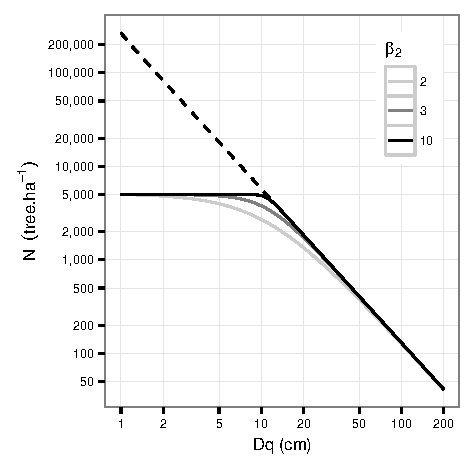
\includegraphics[width=8cm]{fig1.pdf}
	\caption{$\beta_2$ as a shape parameter. Solid lines represent $N$ trajectories with an initial density of 5000 tree per ha while the dashed line is the self-thinning line. Parameter values for $\beta_0$ and $\beta_1$ used to simulate trajectories were computed by fixing $intercept$ and $slope$ of the self-thinning line to known values (12.46 and -1.65, respectively) and then varying $\beta_2$. $\beta_1$, then  $\beta_0$ were derived by rearranging Eqs.\ref{eq:intercept} and \ref{eq:slope} (cf. Appendix)}
	\label{fig:fig1}
\end{figure}

\begin{figure}%[!htbp]
	\centering
	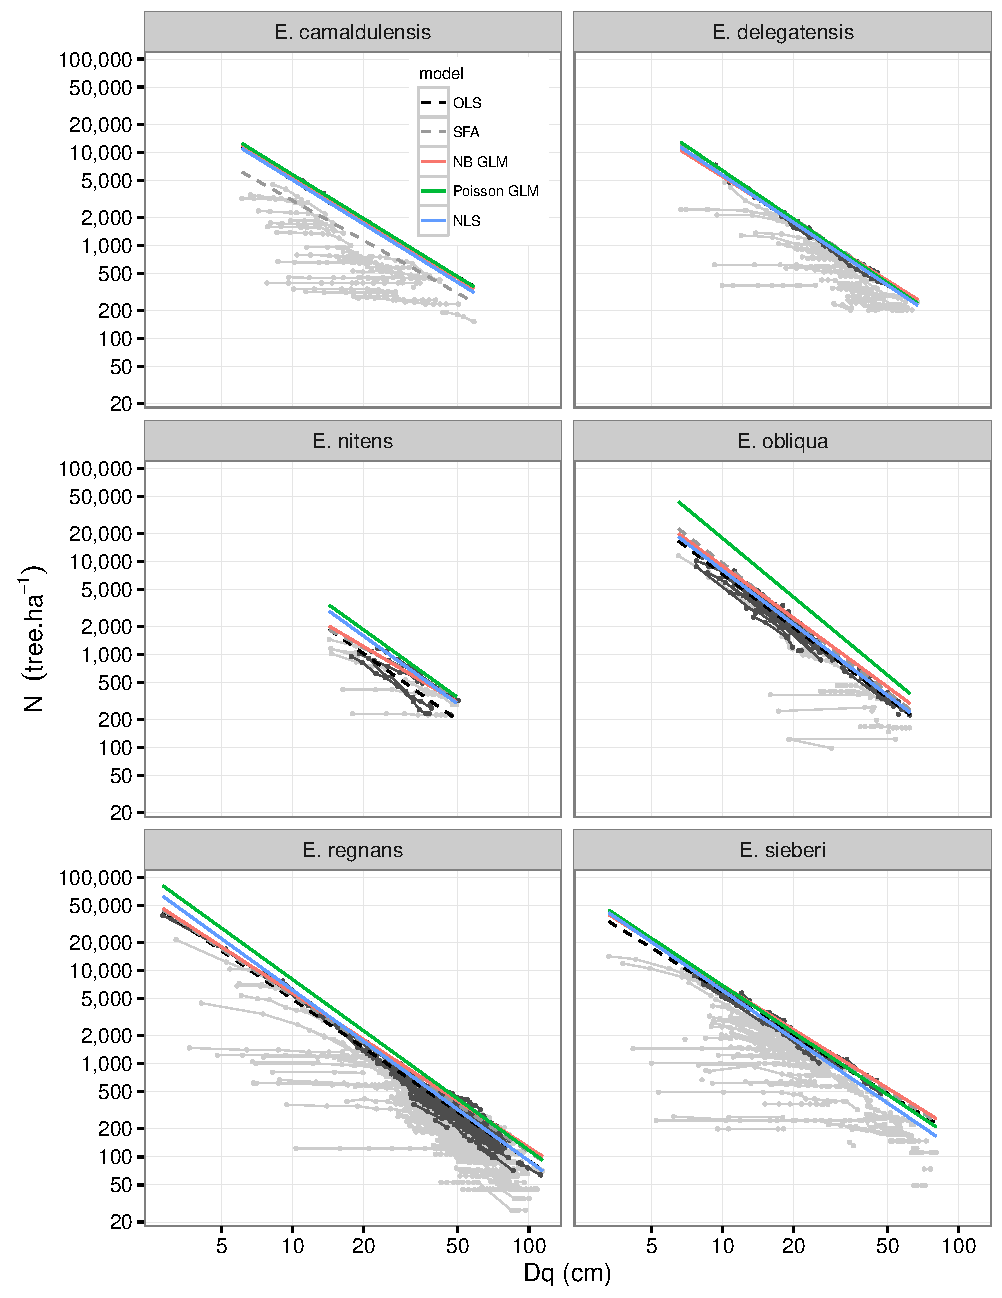
\includegraphics[width=16cm]{fig2.pdf}
	\caption{Estimated self-thinning line for each of the 6 species. Black and grey dots show inventories for control and non-control plots, respectively. Connecting solid lines are plot trajectories}
	\label{fig:fig2}
\end{figure}
\begin{figure}%[!htbp]%[H]%[h], [!h]
	\centering
	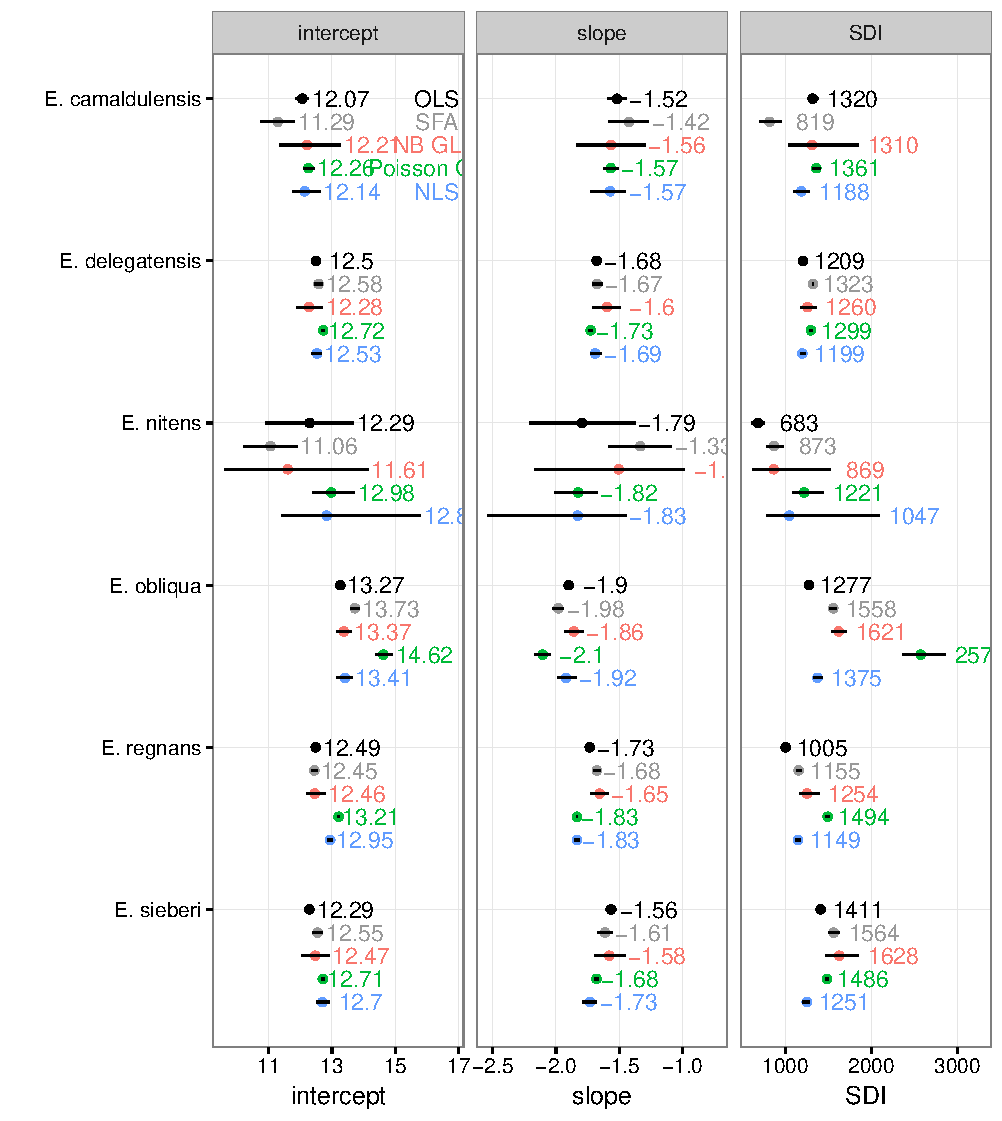
\includegraphics[width=16cm]{fig3.pdf}
	\caption{Point estimates and 95\% CI for the intercept and the slope of the self-thinning line}
	\label{fig:fig3}
\end{figure} 

\begin{figure}%[!htbp]%[H]%[h], [!h]
	\centering
	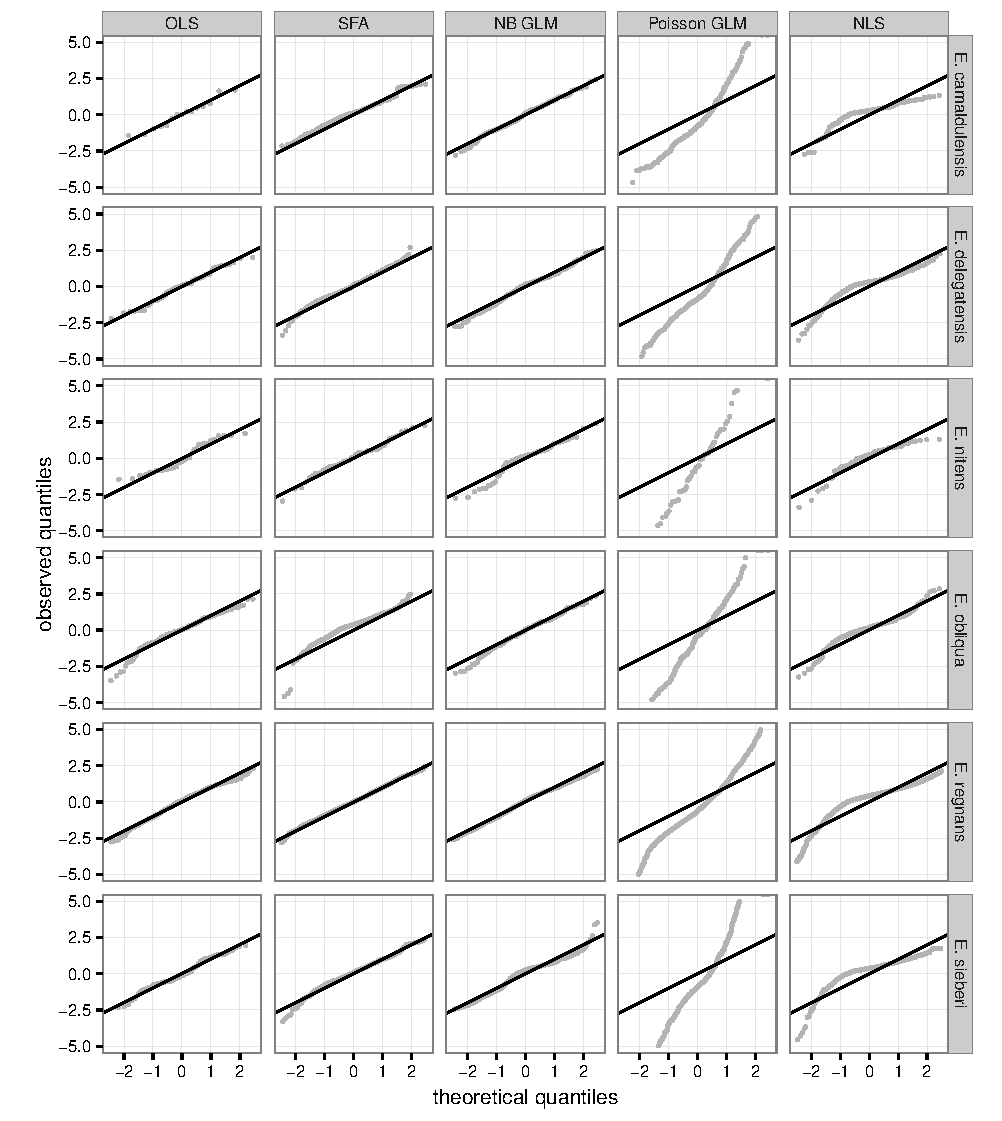
\includegraphics[width=16cm]{fig4.pdf}
	\caption{Residual quantile-quantile plots for the 6 species and 5 models}
	\label{fig:qqplot}
\end{figure}
	
\begin{figure}%[!htbp]%[H]%[h], [!h]
	\centering
	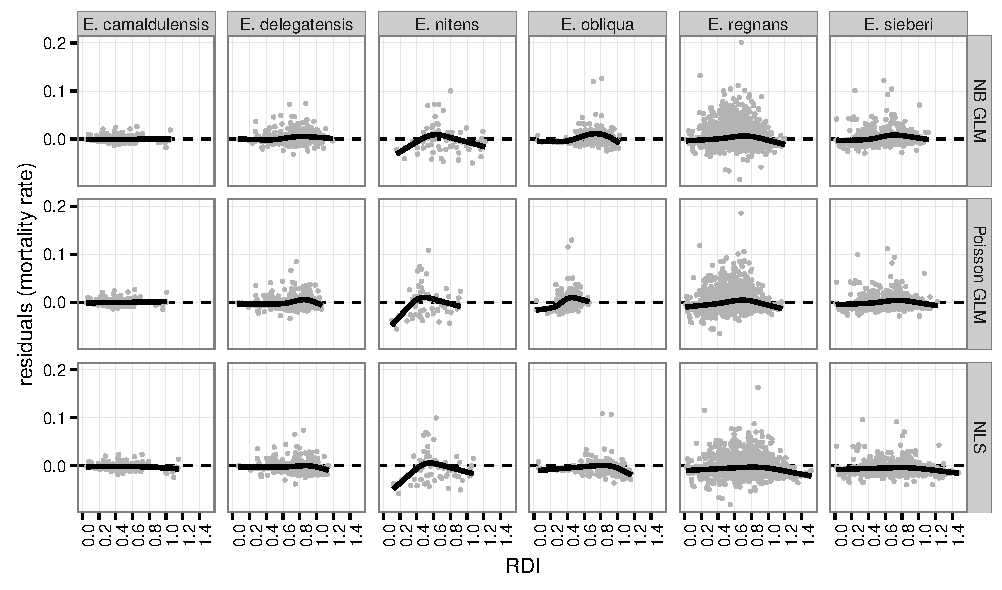
\includegraphics[width=16cm]{fig5.pdf}
	\caption{Residuals against RDI values for the 6 species and 3 mortality models}
	\label{fig:res_rdi}
\end{figure}
	
\begin{figure}%[!htbp]%[H]
	\centering
	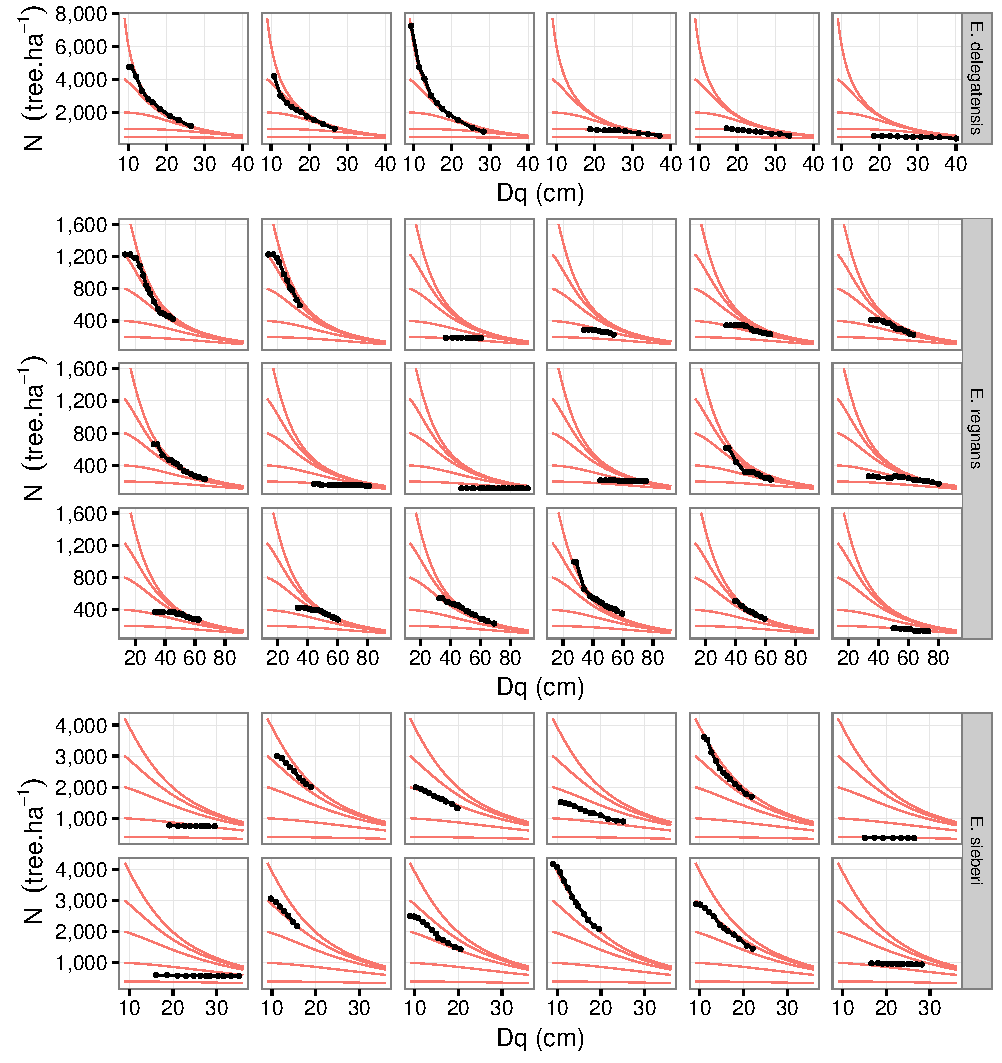
\includegraphics[width=16cm]{fig6.pdf}
	\caption{Observed and predicted trajectories on a validation serie with contrasting silvicultural conditions. Negative binomial GLM for each species (table \ref{tab:parameters}) was used to forecast $N$ trajectories. Black dots and lines are trajectories for one plot. Solid red lines show predictions for different N starting values. Validations predictions for poisson GLM and NLS are available in \textbf{Appendix A}}
	\label{fig:validation}
\end{figure}


\newpage
\begin{sidewaystable}
	\caption{Summary statistics of the data}
	\resizebox{.88\textwidth}{!}{\begin{minipage}{\textwidth} %0.88
			\label{tab:table_material_V2}
			\begin{tabular}{llccccccccccccccccc}
\toprule
& & serie & plot & inventory & \multicolumn{2}{c}{period ($year$)} & \multicolumn{2}{c}{area ($m^2$)} & \multicolumn{2}{c}{elevation ($m$)} & \multicolumn{2}{c}{age ($year$)} & \multicolumn{2}{c}{Dq ($cm$)} & \multicolumn{2}{c}{N ($tree.ha^{-1}$)} & \multicolumn{2}{c}{BA ($m^2.ha^{-1}$)} \\ \cmidrule(lr){6-7}\cmidrule(lr){8-9}\cmidrule(lr){10-11}\cmidrule(lr){12-13}\cmidrule(lr){14-15}\cmidrule(lr){16-17}\cmidrule(lr){18-19}
 &  & n & n & n & mean & sd & mean & sd & mean & sd & mean & range & mean & range & mean & range & mean & \multicolumn{1}{c}{range} \\ 
\midrule
\multicolumn{3}{l}{E. camaldulensis} \\  & SFA  & 4 & 30 & 236 & 4.6 & \multicolumn{1}{l@{}}{2.8} & 850 & \multicolumn{1}{l@{}}{753} & 60 & \multicolumn{1}{l@{}}{0} & 38 & \multicolumn{1}{l@{}}{(9-117)} & 21 & \multicolumn{1}{l@{}}{(6-59)} & 1068 & \multicolumn{1}{l@{}}{(112-5513)} & 23 & \multicolumn{1}{l@{}}{(2-64)} \\
 & OLS  & 1 & 3 & 15 & 4.2 & \multicolumn{1}{l@{}}{2.8} & 801 & \multicolumn{1}{l@{}}{7} & 60 & \multicolumn{1}{l@{}}{0} & 40 & \multicolumn{1}{l@{}}{(27-69)} & 15 & \multicolumn{1}{l@{}}{(9-26)} & 3382 & \multicolumn{1}{l@{}}{(1195-5513)} & 50 & \multicolumn{1}{l@{}}{(39-64)} \\
 & mortality  & 4 & 30 & 193 & 4.8 & \multicolumn{1}{l@{}}{2.8} & 851 & \multicolumn{1}{l@{}}{749} & 60 & \multicolumn{1}{l@{}}{0} & 32 & \multicolumn{1}{l@{}}{(9-70)} & 19 & \multicolumn{1}{l@{}}{(6-53)} & 1118 & \multicolumn{1}{l@{}}{(171-5513)} & 22 & \multicolumn{1}{l@{}}{(2-61)} \\
 & validation  &  &  &  &  & \multicolumn{1}{l@{}}{} &  & \multicolumn{1}{l@{}}{} &  & \multicolumn{1}{l@{}}{} &  & \multicolumn{1}{l@{}}{} &  & \multicolumn{1}{l@{}}{} &  & \multicolumn{1}{l@{}}{} &  & \multicolumn{1}{l@{}}{} \\
\multicolumn{3}{l}{E. delegatensis} \\  & SFA  & 10 & 45 & 384 & 2.4 & \multicolumn{1}{l@{}}{0.8} & 1782 & \multicolumn{1}{l@{}}{1016} & 1040 & \multicolumn{1}{l@{}}{222} & 32 & \multicolumn{1}{l@{}}{(4-70)} & 33 & \multicolumn{1}{l@{}}{(7-67)} & 765 & \multicolumn{1}{l@{}}{(201-7259)} & 45 & \multicolumn{1}{l@{}}{(3-87)} \\
 & OLS  & 6 & 11 & 68 & 2.5 & \multicolumn{1}{l@{}}{0.8} & 1833 & \multicolumn{1}{l@{}}{1147} & 1066 & \multicolumn{1}{l@{}}{159} & 35 & \multicolumn{1}{l@{}}{(13-58)} & 31 & \multicolumn{1}{l@{}}{(9-63)} & 1362 & \multicolumn{1}{l@{}}{(272-7259)} & 63 & \multicolumn{1}{l@{}}{(43-85)} \\
 & mortality  & 10 & 44 & 343 & 2.4 & \multicolumn{1}{l@{}}{0.8} & 1830 & \multicolumn{1}{l@{}}{1029} & 1067 & \multicolumn{1}{l@{}}{229} & 31 & \multicolumn{1}{l@{}}{(4-69)} & 33 & \multicolumn{1}{l@{}}{(7-64)} & 783 & \multicolumn{1}{l@{}}{(201-7259)} & 44 & \multicolumn{1}{l@{}}{(3-84)} \\
 & validation  & 1 & 6 & 60 & 2.8 & \multicolumn{1}{l@{}}{1} & 405 & \multicolumn{1}{l@{}}{0} & 1200 & \multicolumn{1}{l@{}}{0} & 23 & \multicolumn{1}{l@{}}{(13-34)} & 22 & \multicolumn{1}{l@{}}{(9-40)} & 1707 & \multicolumn{1}{l@{}}{(420-7259)} & 45 & \multicolumn{1}{l@{}}{(15-65)} \\
\multicolumn{3}{l}{E. nitens} \\  & SFA  & 4 & 13 & 77 & 2.3 & \multicolumn{1}{l@{}}{0.8} & 901 & \multicolumn{1}{l@{}}{436} & 534 & \multicolumn{1}{l@{}}{195} & 17 & \multicolumn{1}{l@{}}{(5-39)} & 30 & \multicolumn{1}{l@{}}{(14-50)} & 579 & \multicolumn{1}{l@{}}{(224-1445)} & 35 & \multicolumn{1}{l@{}}{(6-64)} \\
 & OLS  & 4 & 7 & 40 & 2.5 & \multicolumn{1}{l@{}}{1.1} & 761 & \multicolumn{1}{l@{}}{470} & 451 & \multicolumn{1}{l@{}}{185} & 20 & \multicolumn{1}{l@{}}{(10-39)} & 30 & \multicolumn{1}{l@{}}{(18-50)} & 608 & \multicolumn{1}{l@{}}{(224-1156)} & 39 & \multicolumn{1}{l@{}}{(24-64)} \\
 & mortality  & 4 & 13 & 64 & 2.3 & \multicolumn{1}{l@{}}{0.8} & 884 & \multicolumn{1}{l@{}}{411} & 527 & \multicolumn{1}{l@{}}{198} & 16 & \multicolumn{1}{l@{}}{(5-35)} & 29 & \multicolumn{1}{l@{}}{(14-48)} & 596 & \multicolumn{1}{l@{}}{(225-1445)} & 34 & \multicolumn{1}{l@{}}{(6-59)} \\
 & validation  &  &  &  &  & \multicolumn{1}{l@{}}{} &  & \multicolumn{1}{l@{}}{} &  & \multicolumn{1}{l@{}}{} &  & \multicolumn{1}{l@{}}{} &  & \multicolumn{1}{l@{}}{} &  & \multicolumn{1}{l@{}}{} &  & \multicolumn{1}{l@{}}{} \\
\multicolumn{3}{l}{E. obliqua} \\  & SFA  & 9 & 111 & 322 & 4.1 & \multicolumn{1}{l@{}}{4.7} & 1011 & \multicolumn{1}{l@{}}{884} & 722 & \multicolumn{1}{l@{}}{143} & 36 & \multicolumn{1}{l@{}}{(13-91)} & 25 & \multicolumn{1}{l@{}}{(6-62)} & 2329 & \multicolumn{1}{l@{}}{(99-11475)} & 56 & \multicolumn{1}{l@{}}{(4-86)} \\
 & OLS  & 5 & 84 & 221 & 3.2 & \multicolumn{1}{l@{}}{1.2} & 970 & \multicolumn{1}{l@{}}{936} & 788 & \multicolumn{1}{l@{}}{63} & 35 & \multicolumn{1}{l@{}}{(13-91)} & 22 & \multicolumn{1}{l@{}}{(8-62)} & 2813 & \multicolumn{1}{l@{}}{(224-11100)} & 61 & \multicolumn{1}{l@{}}{(36-86)} \\
 & mortality  & 9 & 95 & 198 & 3.8 & \multicolumn{1}{l@{}}{3.1} & 1068 & \multicolumn{1}{l@{}}{877} & 703 & \multicolumn{1}{l@{}}{156} & 34 & \multicolumn{1}{l@{}}{(13-86)} & 23 & \multicolumn{1}{l@{}}{(6-60)} & 2713 & \multicolumn{1}{l@{}}{(123-11475)} & 55 & \multicolumn{1}{l@{}}{(4-80)} \\
 & validation  &  &  &  &  & \multicolumn{1}{l@{}}{} &  & \multicolumn{1}{l@{}}{} &  & \multicolumn{1}{l@{}}{} &  & \multicolumn{1}{l@{}}{} &  & \multicolumn{1}{l@{}}{} &  & \multicolumn{1}{l@{}}{} &  & \multicolumn{1}{l@{}}{} \\
\multicolumn{3}{l}{E. regnans} \\  & SFA  & 24 & 185 & 2373 & 2.5 & \multicolumn{1}{l@{}}{1.3} & 2167 & \multicolumn{1}{l@{}}{1466} & 621 & \multicolumn{1}{l@{}}{189} & 43 & \multicolumn{1}{l@{}}{(3-118)} & 50 & \multicolumn{1}{l@{}}{(3-114)} & 452 & \multicolumn{1}{l@{}}{(27-39288)} & 44 & \multicolumn{1}{l@{}}{(1-100)} \\
 & OLS  & 19 & 77 & 677 & 2.7 & \multicolumn{1}{l@{}}{1.6} & 1653 & \multicolumn{1}{l@{}}{1108} & 638 & \multicolumn{1}{l@{}}{187} & 48 & \multicolumn{1}{l@{}}{(4-118)} & 48 & \multicolumn{1}{l@{}}{(3-112)} & 696 & \multicolumn{1}{l@{}}{(64-39288)} & 59 & \multicolumn{1}{l@{}}{(25-99)} \\
 & mortality  & 24 & 185 & 2118 & 2.6 & \multicolumn{1}{l@{}}{1.4} & 2154 & \multicolumn{1}{l@{}}{1466} & 626 & \multicolumn{1}{l@{}}{187} & 42 & \multicolumn{1}{l@{}}{(3-107)} & 48 & \multicolumn{1}{l@{}}{(3-111)} & 458 & \multicolumn{1}{l@{}}{(27-39288)} & 43 & \multicolumn{1}{l@{}}{(1-99)} \\
 & validation  & 1 & 18 & 285 & 2.7 & \multicolumn{1}{l@{}}{0.9} & 1290 & \multicolumn{1}{l@{}}{305} & 778 & \multicolumn{1}{l@{}}{57} & 48 & \multicolumn{1}{l@{}}{(8-81)} & 51 & \multicolumn{1}{l@{}}{(13-92)} & 355 & \multicolumn{1}{l@{}}{(115-1225)} & 60 & \multicolumn{1}{l@{}}{(17-99)} \\
\multicolumn{3}{l}{E. sieberi} \\  & SFA  & 13 & 114 & 639 & 2.8 & \multicolumn{1}{l@{}}{1.4} & 1143 & \multicolumn{1}{l@{}}{764} & 330 & \multicolumn{1}{l@{}}{64} & 37 & \multicolumn{1}{l@{}}{(4-102)} & 26 & \multicolumn{1}{l@{}}{(3-80)} & 1649 & \multicolumn{1}{l@{}}{(49-14247)} & 41 & \multicolumn{1}{l@{}}{(1-105)} \\
 & OLS  & 8 & 31 & 108 & 3.4 & \multicolumn{1}{l@{}}{1.4} & 1011 & \multicolumn{1}{l@{}}{694} & 342 & \multicolumn{1}{l@{}}{95} & 39 & \multicolumn{1}{l@{}}{(14-102)} & 21 & \multicolumn{1}{l@{}}{(8-47)} & 2851 & \multicolumn{1}{l@{}}{(478-9525)} & 63 & \multicolumn{1}{l@{}}{(38-105)} \\
 & mortality  & 12 & 106 & 521 & 2.8 & \multicolumn{1}{l@{}}{1.3} & 1164 & \multicolumn{1}{l@{}}{747} & 331 & \multicolumn{1}{l@{}}{64} & 36 & \multicolumn{1}{l@{}}{(4-92)} & 26 & \multicolumn{1}{l@{}}{(3-79)} & 1679 & \multicolumn{1}{l@{}}{(49-14247)} & 40 & \multicolumn{1}{l@{}}{(1-99)} \\
 & validation  & 1 & 12 & 126 & 2.3 & \multicolumn{1}{l@{}}{0.4} & 1733 & \multicolumn{1}{l@{}}{94} & 280 & \multicolumn{1}{l@{}}{0} & 31 & \multicolumn{1}{l@{}}{(21-47)} & 18 & \multicolumn{1}{l@{}}{(9-35)} & 1737 & \multicolumn{1}{l@{}}{(364-4169)} & 36 & \multicolumn{1}{l@{}}{(7-64)} \\
\bottomrule 
\end{tabular}

	\end{minipage}}
\end{sidewaystable}

\begin{table}
    \caption{Parameter point estimates of the models. 95\% confidence intervals (self-thinning) and standard errors (mortality) are shown under brackets}    
    \resizebox{.65\textwidth}{!}{\begin{minipage}{\textwidth}						
    	\label{tab:parameters}
    	\begin{tabular}{llccccccccccccccc}
\toprule
& & \multicolumn{6}{c}{self-thinning} & \multicolumn{6}{c}{mortality} & \multicolumn{3}{c}{error distribution} \\ \cmidrule(lr){3-8}\cmidrule(lr){9-14}\cmidrule(lr){15-17}
 &  & intercept &  & slope &  & SDI &  & $\beta_0$ &  & $\beta_1$ &  & $\beta_2$ &  & $\sigma$ & $\sigma_U$ & \multicolumn{1}{c}{$\theta$} \\ 
\midrule
\multicolumn{3}{l}{E. camaldulensis} \\  & OLS  & \multicolumn{1}{r@{}}{12.07} & (11.86, 12.28) & \multicolumn{1}{r@{}}{-1.52} & (-1.59, -1.44) & \multicolumn{1}{r@{}}{1320} & (1257, 1385) & \multicolumn{1}{r@{}}{} &  & \multicolumn{1}{r@{}}{} &  & \multicolumn{1}{r@{}}{} &  & 0.04 &  &  \\
 & SFA  & \multicolumn{1}{r@{}}{11.29} & (10.76, 11.83) & \multicolumn{1}{r@{}}{-1.42} & (-1.58, -1.27) & \multicolumn{1}{r@{}}{819} & (706, 953) & \multicolumn{1}{r@{}}{} &  & \multicolumn{1}{r@{}}{} &  & \multicolumn{1}{r@{}}{} &  & 0.44 & 0.78 &  \\
 & NB GLM  & \multicolumn{1}{r@{}}{12.21} & (11.34, 13.28) & \multicolumn{1}{r@{}}{-1.56} & (-1.84, -1.3) & \multicolumn{1}{r@{}}{1310} & (1041, 1853) & \multicolumn{1}{r@{}}{-22.7} & (2.54) & \multicolumn{1}{r@{}}{1.96} & (0.41) & \multicolumn{1}{r@{}}{2.9} & (0.23) &  &  & 0.43 \\
 & Poisson GLM  & \multicolumn{1}{r@{}}{12.26} & (12.09, 12.44) & \multicolumn{1}{r@{}}{-1.57} & (-1.63, -1.51) & \multicolumn{1}{r@{}}{1361} & (1314, 1409) & \multicolumn{1}{r@{}}{-22.08} & (0.49) & \multicolumn{1}{r@{}}{1.88} & (0.08) & \multicolumn{1}{r@{}}{2.84} & (0.04) &  &  &  \\
 & NLS  & \multicolumn{1}{r@{}}{12.14} & (11.76, 12.63) & \multicolumn{1}{r@{}}{-1.57} & (-1.73, -1.45) & \multicolumn{1}{r@{}}{1188} & (1099, 1288) & \multicolumn{1}{r@{}}{-20.91} & (1.95) & \multicolumn{1}{r@{}}{1.77} & (0.29) & \multicolumn{1}{r@{}}{2.76} & (0.16) & 0.05 &  &  \\
\multicolumn{3}{l}{E. delegatensis} \\  & OLS  & \multicolumn{1}{r@{}}{12.5} & (12.38, 12.62) & \multicolumn{1}{r@{}}{-1.68} & (-1.71, -1.64) & \multicolumn{1}{r@{}}{1209} & (1189, 1229) & \multicolumn{1}{r@{}}{} &  & \multicolumn{1}{r@{}}{} &  & \multicolumn{1}{r@{}}{} &  & 0.07 &  &  \\
 & SFA  & \multicolumn{1}{r@{}}{12.58} & (12.46, 12.7) & \multicolumn{1}{r@{}}{-1.67} & (-1.71, -1.64) & \multicolumn{1}{r@{}}{1323} & (1314, 1333) & \multicolumn{1}{r@{}}{} &  & \multicolumn{1}{r@{}}{} &  & \multicolumn{1}{r@{}}{} &  & 0.04 & 0.68 &  \\
 & NB GLM  & \multicolumn{1}{r@{}}{12.28} & (11.89, 12.71) & \multicolumn{1}{r@{}}{-1.6} & (-1.71, -1.49) & \multicolumn{1}{r@{}}{1260} & (1172, 1362) & \multicolumn{1}{r@{}}{-35.5} & (2.37) & \multicolumn{1}{r@{}}{3.68} & (0.35) & \multicolumn{1}{r@{}}{3.93} & (0.19) &  &  & 0.95 \\
 & Poisson GLM  & \multicolumn{1}{r@{}}{12.72} & (12.67, 12.77) & \multicolumn{1}{r@{}}{-1.73} & (-1.74, -1.71) & \multicolumn{1}{r@{}}{1299} & (1286, 1313) & \multicolumn{1}{r@{}}{-31.23} & (0.53) & \multicolumn{1}{r@{}}{3.31} & (0.08) & \multicolumn{1}{r@{}}{3.5} & (0.04) &  &  &  \\
 & NLS  & \multicolumn{1}{r@{}}{12.53} & (12.35, 12.66) & \multicolumn{1}{r@{}}{-1.69} & (-1.73, -1.64) & \multicolumn{1}{r@{}}{1199} & (1175, 1232) & \multicolumn{1}{r@{}}{-34.43} & (2.28) & \multicolumn{1}{r@{}}{3.71} & (0.32) & \multicolumn{1}{r@{}}{3.79} & (0.18) & 0.04 &  &  \\
\multicolumn{3}{l}{E. nitens} \\  & OLS  & \multicolumn{1}{r@{}}{12.29} & (10.89, 13.69) & \multicolumn{1}{r@{}}{-1.79} & (-2.21, -1.37) & \multicolumn{1}{r@{}}{683} & (611, 763) & \multicolumn{1}{r@{}}{} &  & \multicolumn{1}{r@{}}{} &  & \multicolumn{1}{r@{}}{} &  & 0.28 &  &  \\
 & SFA  & \multicolumn{1}{r@{}}{11.06} & (10.22, 11.9) & \multicolumn{1}{r@{}}{-1.33} & (-1.58, -1.08) & \multicolumn{1}{r@{}}{873} & (780, 977) & \multicolumn{1}{r@{}}{} &  & \multicolumn{1}{r@{}}{} &  & \multicolumn{1}{r@{}}{} &  & 0.16 & 0.54 &  \\
 & NB GLM  & \multicolumn{1}{r@{}}{11.61} & (9.6, 14.14) & \multicolumn{1}{r@{}}{-1.5} & (-2.17, -0.98) & \multicolumn{1}{r@{}}{869} & (615, 1531) & \multicolumn{1}{r@{}}{-18.84} & (4.1) & \multicolumn{1}{r@{}}{1.49} & (0.63) & \multicolumn{1}{r@{}}{2.66} & (0.38) &  &  & 0.89 \\
 & Poisson GLM  & \multicolumn{1}{r@{}}{12.98} & (12.4, 13.72) & \multicolumn{1}{r@{}}{-1.82} & (-2.01, -1.67) & \multicolumn{1}{r@{}}{1221} & (1083, 1448) & \multicolumn{1}{r@{}}{-14.02} & (0.83) & \multicolumn{1}{r@{}}{1.05} & (0.11) & \multicolumn{1}{r@{}}{2.13} & (0.08) &  &  &  \\
 & NLS  & \multicolumn{1}{r@{}}{12.84} & (11.4, 15.81) & \multicolumn{1}{r@{}}{-1.83} & (-2.54, -1.45) & \multicolumn{1}{r@{}}{1047} & (782, 2100) & \multicolumn{1}{r@{}}{-15.01} & (3.41) & \multicolumn{1}{r@{}}{1.22} & (0.46) & \multicolumn{1}{r@{}}{2.22} & (0.32) & 0.08 &  &  \\
\multicolumn{3}{l}{E. obliqua} \\  & OLS  & \multicolumn{1}{r@{}}{13.27} & (13.15, 13.38) & \multicolumn{1}{r@{}}{-1.9} & (-1.94, -1.86) & \multicolumn{1}{r@{}}{1277} & (1252, 1304) & \multicolumn{1}{r@{}}{} &  & \multicolumn{1}{r@{}}{} &  & \multicolumn{1}{r@{}}{} &  & 0.14 &  &  \\
 & SFA  & \multicolumn{1}{r@{}}{13.73} & (13.59, 13.86) & \multicolumn{1}{r@{}}{-1.98} & (-2.02, -1.94) & \multicolumn{1}{r@{}}{1558} & (1518, 1599) & \multicolumn{1}{r@{}}{} &  & \multicolumn{1}{r@{}}{} &  & \multicolumn{1}{r@{}}{} &  & 0.06 & 0.54 &  \\
 & NB GLM  & \multicolumn{1}{r@{}}{13.37} & (13.13, 13.6) & \multicolumn{1}{r@{}}{-1.86} & (-1.93, -1.78) & \multicolumn{1}{r@{}}{1621} & (1543, 1713) & \multicolumn{1}{r@{}}{-20.72} & (1.71) & \multicolumn{1}{r@{}}{1.97} & (0.26) & \multicolumn{1}{r@{}}{2.6} & (0.13) &  &  & 10.68 \\
 & Poisson GLM  & \multicolumn{1}{r@{}}{14.62} & (14.37, 14.91) & \multicolumn{1}{r@{}}{-2.1} & (-2.17, -2.04) & \multicolumn{1}{r@{}}{2573} & (2368, 2863) & \multicolumn{1}{r@{}}{-8.02} & (0.41) & \multicolumn{1}{r@{}}{0.26} & (0.06) & \multicolumn{1}{r@{}}{1.6} & (0.03) &  &  &  \\
 & NLS  & \multicolumn{1}{r@{}}{13.41} & (13.15, 13.64) & \multicolumn{1}{r@{}}{-1.92} & (-1.99, -1.84) & \multicolumn{1}{r@{}}{1375} & (1333, 1430) & \multicolumn{1}{r@{}}{-20.33} & (1.97) & \multicolumn{1}{r@{}}{2.01} & (0.29) & \multicolumn{1}{r@{}}{2.57} & (0.15) & 0.06 &  &  \\
\multicolumn{3}{l}{E. regnans} \\  & OLS  & \multicolumn{1}{r@{}}{12.49} & (12.36, 12.62) & \multicolumn{1}{r@{}}{-1.73} & (-1.77, -1.7) & \multicolumn{1}{r@{}}{1005} & (980, 1030) & \multicolumn{1}{r@{}}{} &  & \multicolumn{1}{r@{}}{} &  & \multicolumn{1}{r@{}}{} &  & 0.19 &  &  \\
 & SFA  & \multicolumn{1}{r@{}}{12.45} & (12.35, 12.55) & \multicolumn{1}{r@{}}{-1.68} & (-1.7, -1.65) & \multicolumn{1}{r@{}}{1155} & (1127, 1184) & \multicolumn{1}{r@{}}{} &  & \multicolumn{1}{r@{}}{} &  & \multicolumn{1}{r@{}}{} &  & 0.13 & 0.71 &  \\
 & NB GLM  & \multicolumn{1}{r@{}}{12.46} & (12.18, 12.79) & \multicolumn{1}{r@{}}{-1.65} & (-1.73, -1.59) & \multicolumn{1}{r@{}}{1254} & (1162, 1393) & \multicolumn{1}{r@{}}{-20.95} & (0.85) & \multicolumn{1}{r@{}}{1.85} & (0.12) & \multicolumn{1}{r@{}}{2.72} & (0.07) &  &  & 0.85 \\
 & Poisson GLM  & \multicolumn{1}{r@{}}{13.21} & (13.18, 13.24) & \multicolumn{1}{r@{}}{-1.83} & (-1.84, -1.83) & \multicolumn{1}{r@{}}{1494} & (1473, 1515) & \multicolumn{1}{r@{}}{-16.16} & (0.17) & \multicolumn{1}{r@{}}{1.33} & (0.02) & \multicolumn{1}{r@{}}{2.27} & (0.01) &  &  &  \\
 & NLS  & \multicolumn{1}{r@{}}{12.95} & (12.86, 13.03) & \multicolumn{1}{r@{}}{-1.83} & (-1.85, -1.81) & \multicolumn{1}{r@{}}{1149} & (1119, 1179) & \multicolumn{1}{r@{}}{-18.21} & (0.64) & \multicolumn{1}{r@{}}{1.66} & (0.09) & \multicolumn{1}{r@{}}{2.45} & (0.05) & 0.05 &  &  \\
\multicolumn{3}{l}{E. sieberi} \\  & OLS  & \multicolumn{1}{r@{}}{12.29} & (12.15, 12.43) & \multicolumn{1}{r@{}}{-1.56} & (-1.61, -1.52) & \multicolumn{1}{r@{}}{1411} & (1376, 1447) & \multicolumn{1}{r@{}}{} &  & \multicolumn{1}{r@{}}{} &  & \multicolumn{1}{r@{}}{} &  & 0.11 &  &  \\
 & SFA  & \multicolumn{1}{r@{}}{12.55} & (12.37, 12.72) & \multicolumn{1}{r@{}}{-1.61} & (-1.67, -1.55) & \multicolumn{1}{r@{}}{1564} & (1499, 1632) & \multicolumn{1}{r@{}}{} &  & \multicolumn{1}{r@{}}{} &  & \multicolumn{1}{r@{}}{} &  & 0.09 & 0.98 &  \\
 & NB GLM  & \multicolumn{1}{r@{}}{12.47} & (12.04, 12.92) & \multicolumn{1}{r@{}}{-1.58} & (-1.7, -1.45) & \multicolumn{1}{r@{}}{1628} & (1465, 1856) & \multicolumn{1}{r@{}}{-18.14} & (1.14) & \multicolumn{1}{r@{}}{1.35} & (0.17) & \multicolumn{1}{r@{}}{2.49} & (0.1) &  &  & 0.75 \\
 & Poisson GLM  & \multicolumn{1}{r@{}}{12.71} & (12.67, 12.75) & \multicolumn{1}{r@{}}{-1.68} & (-1.69, -1.67) & \multicolumn{1}{r@{}}{1486} & (1470, 1502) & \multicolumn{1}{r@{}}{-18.76} & (0.2) & \multicolumn{1}{r@{}}{1.55} & (0.03) & \multicolumn{1}{r@{}}{2.52} & (0.02) &  &  &  \\
 & NLS  & \multicolumn{1}{r@{}}{12.7} & (12.53, 12.91) & \multicolumn{1}{r@{}}{-1.73} & (-1.79, -1.68) & \multicolumn{1}{r@{}}{1251} & (1205, 1285) & \multicolumn{1}{r@{}}{-18.19} & (1.08) & \multicolumn{1}{r@{}}{1.55} & (0.15) & \multicolumn{1}{r@{}}{2.48} & (0.09) & 0.05 &  &  \\
\bottomrule 
\end{tabular}

    \end{minipage}}
\end{table}
    	
	\begin{table}%[!htbp]%[H]
		\centering
		\caption{Mortality models goodness-of-fit on calibration dataset}						
		\label{tab:gof_cal}
		\begin{tabular}{llcccccc}
\toprule
& & \multicolumn{3}{c}{mortality count} & \multicolumn{3}{c}{mortality rate} \\ \cmidrule(lr){3-5}\cmidrule(lr){6-8}
 &  & $R^2$ & $RMSE$ & $BIAS$ & $R^2$ & $RMSE$ & \multicolumn{1}{c}{$BIAS$} \\ 
\midrule
\multicolumn{2}{l}{E. camaldulensis} \\  & NB GLM  & $0.83$ & $\phantom{-}13.9$ & $\phantom{0}-0.4$ & $0.56$ & $0.006$ & $-0.001$ \\
 & Poisson GLM  & $0.84$ & $\phantom{-}13.4$ & $\phantom{0}\phantom{-}0.2$ & $0.57$ & $0.006$ & $\phantom{-}0.000$ \\
 & NLS  & $0.75$ & $\phantom{-}16.8$ & $\phantom{0}-3.4$ & $0.46$ & $0.007$ & $-0.002$ \\
\multicolumn{2}{l}{E. delegatensis} \\  & NB GLM  & $0.94$ & $\phantom{-}23.7$ & $\phantom{0}\phantom{-}2.1$ & $0.75$ & $0.013$ & $\phantom{-}0.002$ \\
 & Poisson GLM  & $0.91$ & $\phantom{-}27.5$ & $\phantom{0}\phantom{-}2.8$ & $0.75$ & $0.013$ & $\phantom{-}0.000$ \\
 & NLS  & $0.94$ & $\phantom{-}23.1$ & $\phantom{0}-1.0$ & $0.77$ & $0.013$ & $-0.002$ \\
\multicolumn{2}{l}{E. nitens} \\  & NB GLM  & $0.63$ & $\phantom{-}22.5$ & $\phantom{0}-0.8$ & $0.39$ & $0.030$ & $\phantom{-}0.000$ \\
 & Poisson GLM  & $0.68$ & $\phantom{-}20.9$ & $\phantom{0}\phantom{-}1.8$ & $0.37$ & $0.030$ & $\phantom{-}0.001$ \\
 & NLS  & $0.66$ & $\phantom{-}21.4$ & $\phantom{0}-2.1$ & $0.37$ & $0.031$ & $-0.004$ \\
\multicolumn{2}{l}{E. obliqua} \\  & NB GLM  & $0.88$ & $\phantom{-}74.7$ & $\phantom{-}18.9$ & $0.78$ & $0.018$ & $\phantom{-}0.006$ \\
 & Poisson GLM  & $0.89$ & $\phantom{-}72.9$ & $\phantom{-}26.4$ & $0.75$ & $0.019$ & $\phantom{-}0.005$ \\
 & NLS  & $0.89$ & $\phantom{-}71.4$ & $-10.3$ & $0.83$ & $0.016$ & $-0.003$ \\
\multicolumn{2}{l}{E. regnans} \\  & NB GLM  & $0.99$ & $\phantom{-}38.7$ & $\phantom{0}-0.3$ & $0.63$ & $0.019$ & $\phantom{-}0.003$ \\
 & Poisson GLM  & $0.95$ & $\phantom{-}83.4$ & $\phantom{0}\phantom{-}4.1$ & $0.65$ & $0.018$ & $\phantom{-}0.000$ \\
 & NLS  & $0.98$ & $\phantom{-}47.0$ & $\phantom{0}-1.8$ & $0.69$ & $0.017$ & $-0.005$ \\
\multicolumn{2}{l}{E. sieberi} \\  & NB GLM  & $0.91$ & $\phantom{-}46.5$ & $\phantom{0}\phantom{-}7.0$ & $0.66$ & $0.017$ & $\phantom{-}0.002$ \\
 & Poisson GLM  & $0.93$ & $\phantom{-}42.8$ & $\phantom{0}\phantom{-}3.4$ & $0.70$ & $0.016$ & $\phantom{-}0.000$ \\
 & NLS  & $0.91$ & $\phantom{-}48.4$ & $-11.3$ & $0.70$ & $0.016$ & $-0.006$ \\
\bottomrule 
\end{tabular}

	\end{table}
	
	\begin{table}%[!htbp]%[H]
		\centering
		\caption{Mortality models goodness-of-prediction on validation dataset}						
		\label{tab:gof_val}
		\begin{tabular}{llcccccc}
\toprule
& & \multicolumn{3}{c}{mortality count} & \multicolumn{3}{c}{mortality rate} \\ \cmidrule(lr){3-5}\cmidrule(lr){6-8}
 &  & $R^2$ & $RMSE$ & $BIAS$ & $R^2$ & $RMSE$ & \multicolumn{1}{c}{$BIAS$} \\ 
\midrule
\multicolumn{2}{l}{E. delegatensis} \\  & NB GLM  & $0.93$ & $\phantom{-}52.4$ & $\phantom{0}\phantom{-}9.5$ & $0.78$ & $0.018$ & $\phantom{-}0.006$ \\
 & Poisson GLM  & $0.90$ & $\phantom{-}62.1$ & $\phantom{-}19.8$ & $0.75$ & $0.019$ & $\phantom{-}0.007$ \\
 & NLS  & $0.93$ & $\phantom{-}50.8$ & $\phantom{0}\phantom{-}4.7$ & $0.81$ & $0.017$ & $\phantom{-}0.002$ \\
\multicolumn{2}{l}{E. regnans} \\  & NB GLM  & $0.70$ & $\phantom{0}\phantom{-}6.0$ & $\phantom{0}-1.2$ & $0.55$ & $0.011$ & $-0.004$ \\
 & Poisson GLM  & $0.66$ & $\phantom{0}\phantom{-}6.4$ & $\phantom{0}-1.7$ & $0.46$ & $0.012$ & $-0.006$ \\
 & NLS  & $0.54$ & $\phantom{0}\phantom{-}7.4$ & $\phantom{0}-4.2$ & $0.11$ & $0.016$ & $-0.012$ \\
\multicolumn{2}{l}{E. sieberi} \\  & NB GLM  & $0.80$ & $\phantom{-}17.2$ & $\phantom{0}\phantom{-}0.7$ & $0.63$ & $0.008$ & $-0.001$ \\
 & Poisson GLM  & $0.81$ & $\phantom{-}16.7$ & $\phantom{0}-3.1$ & $0.60$ & $0.009$ & $-0.003$ \\
 & NLS  & $0.65$ & $\phantom{-}22.6$ & $-14.1$ & $0.28$ & $0.012$ & $-0.009$ \\
\bottomrule 
\end{tabular}

	\end{table}
	
\end{document}

